\documentclass[english]{sig-alternate-05-2015}
\usepackage[T1]{fontenc}
\usepackage[latin9]{inputenc}
\usepackage{verbatim}

%% without following commands, amsthm complains proof being already defined 
\let\proof\relax
\let\endproof\relax
\usepackage{amsthm}
\usepackage{amstext}
\usepackage{graphicx}

\usepackage{mdwlist} % compact lists

\usepackage{relsize} % relative font sizes
\usepackage{todonotes} % private notes

\usepackage{soul}

\usepackage{hyperref}
\hypersetup{bookmarks=true,bookmarksnumbered=true,pdfstartview=FitB,colorlinks=true,pdfborder=0 0 0}

\usepackage{amsmath}

\usepackage{xspace}

\usepackage[sort&compress]{natbib}

\makeatletter

%%%%%%%%%%%%%%%%%%%%%%%%%%%%%% LyX specific LaTeX commands.
%% Because html converters don't know tabularnewline
\providecommand{\tabularnewline}{\\}
%% A simple dot to overcome graphicx limitations
\newcommand{\lyxdot}{.}


%%%%%%%%%%%%%%%%%%%%%%%%%%%%%% Textclass specific LaTeX commands.
\theoremstyle{plain}
\newtheorem{thm}{\protect\theoremname}
\theoremstyle{definition}
\newtheorem{defn}{\protect\definitionname}

%%%%%%%%%%%%%%%%%%%%%%%%%%%%%% User specified LaTeX commands.
\usepackage{algorithm}


\usepackage{algpseudocode}

\@ifundefined{showcaptionsetup}{}{%
 \PassOptionsToPackage{caption=false}{subfig}}
\usepackage{subfig}
\makeatother

\usepackage{babel}
\providecommand{\definitionname}{Definition}
\providecommand{\theoremname}{Theorem}

\DeclareCaptionType{copyrightbox}
%========== Custom typographic commands ==========
\newcommand{\emailAddr}[1]{\texttt{\smaller {#1}}}
\newcommand{\mailtoLink}[2]{\href{mailto:#2}{\emailAddr{#1}}}
\newcommand{\refSection}[1]{Section~\ref{#1}}
\newcommand{\refsec}[1]{\S~\ref{#1}}
\newcommand{\refequ}[1]{eq.~\eqref{#1}}
\newcommand{\refEquation}[1]{Equation~\eqref{#1}}
\newcommand{\refFigure}[1]{Figure~\ref{#1}}
\newcommand{\reffig}[1]{fig.~\ref{#1}}
\newcommand{\refDefinition}[1]{Definition~\ref{#1}}
\newcommand{\refdef}[1]{defn.~\ref{#1}}
\newcommand{\refAlgorithm}[1]{Algorithm~\ref{#1}}
\newcommand{\refalg}[1]{alg.~\ref{#1}}
\newcommand{\refTable}[1]{Table~\ref{#1}}
\newcommand{\reftab}[1]{table~\ref{#1}}
\newcommand{\refTheorem}[1]{Theorem~\ref{#1}}
\newcommand{\refthm}[1]{thm.~\ref{#1}}

%========== Document Specific commands ==========


\newcommand{\sv}{SV}
\newcommand{\graphname}[1]{\emph{#1}}




\begin{document}

\setcopyright{acmcopyright}

\title{A Fault Tolerant Connected Component Algorithm }

\numberofauthors{1} 
  \author{
  \alignauthor
    Piyush Sao, Oded Green, Chirag Jain, Richard Vuduc \\
      \affaddr{School of Computational Science and Engineering}\\
      \affaddr{Georgia Institute of Technology}\\
      \email{\{piyush3,ogreen3,cjain3,richie\}@gatech.edu}
  %
  % \alignauthor
  %   Xiaoye S. Li\\
  %     \affaddr{Computational Research Division }\\
  %     \affaddr{Lawrence Berkeley National Laboratory}\\
  %     \email{xsli@lbl.gov}
  }


\maketitle

\begin{abstract}
% \todo{redo}
This paper presents a fault tolerant label propagation based graph connect component algorithm, that can converge to correct solution even in presence soft transient faults. 

%
First, we develop a set of conditions on state variables of the algorithm that ensures
convergence to correct solution. We augment the algorithm 
with additional state variable to make verification of these conditions becomes computationally tractable. 
% valid state not defined
 Finally, we add a local correction scheme which ensures 
the algorithm comes to a valid state after a faulty execution. 

%
We present experimental results on wide range of matrices to show that the new algorithm can withstand high fault rates, with minimal storage and computational overhead. Additionally, we present analytical models for overhead of fault detection and correction. 

\end{abstract}


\keywords{Fault-tolerance, Graph-algorithm, Connected Component, Bit-flip}


\section{Introduction}


The exceeding growth of big datasets has created a need for using distributed systems and 
accelerators for real-time analytics, including for graph and social network analytics. Social 
networks such Facebook and Twitter are constantly growing  at time of writing have over #### 
members with **** relationships between these members.
The decrease of transistor sizes and the improved power consumption, as part of Moore's laws, has 
brought a new challenge with it - an increased number of faults due to random bit flipping. This 
problem is very likely to become even more challenging as transistor sizes continue to decrease and 
the power envelope restrictions become even tighter. As larger systems, with a higher thread count, 
become ubiquitous so will the problem of power related faults.

In this work, we tackle the problem of faults in a connected component algorithm that is 
propagation based. We modify the parallel algorithm of Shiloach-Vishkin \cite{shiloachvishkin} and 
make it fault-tolerant by augmenting the data structures used by the algorithm and by adding a 
detection and correction scheme at the end of every iteration. By detecting and correcting the 
error at the end of each iteration we are able to limit the propagation of the error to the 
remainder of the graph in the following iterations.

Main contributions:
* Little overhead when there aren't any faults.
* Same number of iterations as a fault-free execution for reasonable error rates.
* Overhead if rather constant in time until the number of threads is significantly high.
* 




\label{sec:intro}

\section{Fault Model}

%ODED - Citations are missing in this section.
%ODED - what are some of the latest and greatest results in fault tolerant research?


In this paper, a fault includes any instance in which the underlying
hardware deviates from its expected behavior.
We will use the taxonomy of faults outlined by Hoemmen and Heroux~\cite{hoemmen2011reliability}, 
among others, as summarized below.

%
We distinguish \emph{hard faults} and \emph{soft faults}. A hard fault interrupts the program, 
causing it to immediately crash or terminate. This occurs when, for instance, a node or network 
link fails. By contrast, a soft fault does not cause immediate interruption of the program. L1 cache 
bit flips
are a common type of soft fault. 

A particularly insidious manifestation of soft faults is \emph{silent data corruption} (SDC), where 
an soft fault corrupts the intermediate variables of the algorithm without notifying the
application. Such data corruption may propagates and eventually result in incorrect output
masquerading as correct. 

Recently, a number of techniques have been developed for dealing with soft faults in numerical
linear algebra. There is a large and growing literature on so called
\emph{algorithm based fault tolerance} (ABFT), that primarily rely on testing checksum invariants
\cite{huang1984abft,luk1988abft,du2012abft,shantharam2012ftcg}. 
For iterative numerical algorithms, techniques have been developed where 
algorithm can recover from fault by itself, thus obviating need for fault detection and
correction\cite{hoemmen2011reliability,sao2013sscg, elliott2016exploiting}. 
% 

\icomment{Insert Citations}
In contrast to numerical linear algebra---which is characterized by large data parallel floating point 
computation,  the graph computation is characterized by irregular and indirect memory accesses.
While for slow storage
such as DRAM and disk, error correcting codes are deployed and efficient, fast memory 
such as cache and registers still remains unprotected[cite, cite]. Therefore, large scale graph computation is
as susceptible to soft faults as any other computation. 

As far as we know, the issue of fault tolerance 
in graph computation is, so far, addressed only in context of hard fault and they are based on 
check-pointing and restarting method[cite cite]. Checkpoint and restart based method are usually not 
scalable with high fault rates, and are still prone to silent data corruption.  
%
% Soft faults can be further divided into transient or non-
% transient faults. A transient fault is temporary. Examples include temporarily incorrect output from 
% the floating point unit or a momentary bit flip while reading data from mem- ory. By contrast, 
% non-transient faults are permanent. For instance, suppose the input data stored on disk is 
% corrupted. In this case, reading the data may succeed but the data is wrong on every read.

\icomment{Redo the summary}

%
This paper concerns only transient soft faults. Thus, in the consequent, a ``fault'' is a transient 
soft fault unless otherwise noted. When faults cause the output to fall outside acceptable limits, 
we say the algorithm has failed.
For an algorithm to terminate successfully, at least some amount of computation must be done 
reliably. However, in general we do not have control over which operations are done correctly and 
which operations are done incorrectly. In this paper, we will attempt to distinguish algorithmic 
operations that must be performed reliably from those that may be performed unreliably. We refer to 
these different modes of computation as reliable mode (or reliable computation) from unreliable mode 
(or computation), without saying precisely how to implement these modes. The prior work of others 
similarly assumes ``selective reliability'' ~\cite{hoemmen2011reliability}.
\label{sec:fault}

\section{Fault tolerant Label propagation algorithm for graph connected component}
\begin{algorithm}[!t]
\small
\caption{Label propagation algorithm}
\label{alg:SV_ALG}
\begin{algorithmic}[1]
\Require {$G=(V,E)$}

\State Initialization ;
\For {each $v\in V$}
\State	$CC[v]=v; CCp[v]=v$;
\EndFor

\State $NumChange=|V|$
\While{$NumChange>0$};
\State $NumChange\leftarrow 0$
\State MemCpy($CCp$,$CC$,$|V|$)
\For {each $v\in V$}
\For {each $u\in E(v)$}

\If {$CCp[u]<CC[v]$}
\State $CC[v]\leftarrow CCp[u]$
\State NumChanges = NumChanges+1;
\EndIf

\EndFor
\EndFor

\EndWhile 


\end{algorithmic}
\end{algorithm}
%
\begin{algorithm}[!t]
\small
\caption{Fault Tolerant Label propagation algorithm}
\label{alg:FTSV_ALG}
\begin{algorithmic}[1]
\Require {$G=(V,E)$}

\State Initialization ;
\For {each $v\in V$}
	\State	$CC[v]=v; CCp[v]=v, H[v]=v$;
\EndFor

\State $NumChanges=|V|$
\While{$NumChanges>NumCorrections$};
	\State $NumChanges\leftarrow 0$
	\State MemCpy($CCp$,$CC$,$|V|$)
	\For {each $v\in V$}
		\For {each $u\in E(v)$}

			\If {$CCp[u]<CC[v]$}
			\State $CC[v]\leftarrow CCp[u]$
			\State $H[v]\leftarrow u$
			\State $NumChanges = NumChanges+1$;
			\EndIf

		\EndFor
	\EndFor

	\State Fault detection and correction
	\State $NumCorrections=0$
	\For {each $v\in V$}


		\If {$CC[v] \neq CCp[H[v]] | CC[v] > v | H[v] \notin E(v) $}
		\State $NumCorrections = NumCorrections+1$;
		\For {each $u\in E(v)$}

			\If {$CCp[u]<CC[v]$}
			\State $CC[v]\leftarrow CCp[u]$
			\State $H[v]\leftarrow u$
			\EndIf

		\EndFor

		\EndIf


	\EndFor


\EndWhile 


\end{algorithmic}
\end{algorithm}
%
\label{sec:connected}

\section{Results}
\lyxframe{Experimental Setup }

\begin{block}{Machine Parameter}
\begin{center}
\begin{tabular}{l|l}
\toprule
Prop                 & SNB16c       \\
\midrule
Micro-architecture    & Sandy-Bridge  \\
Sockets$\times$Cores & 2$\times$8   \\
Clock Rate           & 2.4GHz       \\
DRAM capacity        & 128GB        \\
DRAM Bandwidth       & 72GB/s      \\
Compiler       		 & Intel ``C'' compiler 15.0.0     \\
\bottomrule
\end{tabular}
\end{center}
\end{block}

\begin{block}{Fault Injection}
\begin{itemize}
\item Fault injection in reading graph data structure and $CC$ array.
\item Each fault injection read is independent
\item Normalized by number of edges in the network
\end{itemize}
\end{block}

\begin{itemize}
\item Test Network: $14^{th}$ DIMACS graph challenge
\end{itemize}
\lyxframeend{}

%%%%%%%%%%%%%%%%%%%%%%%%%%%%%%%%%%%%%%%%%%%%%%%%%%%%%%%%%

\lyxframe{Fault Free Execution Overhead }
\centering
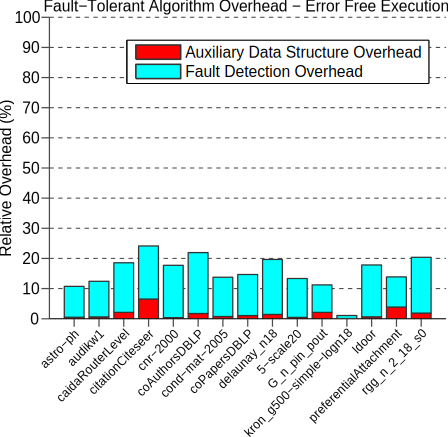
\includegraphics[height=.75\textheight]{plots/plot_zero_overhead-1}

\color{dpg} On an average 1.3\% overhead for maintaining additional data structure and 14\%
for fault detection.
\lyxframeend{}

%%%%%%%%%%%%%%%%%%%%%%%%%%%%%%%%%%%%%%%%%%%%%%%%%%%%%%%%%
\lyxframe{Failure Rate for synchronous case }
\centering
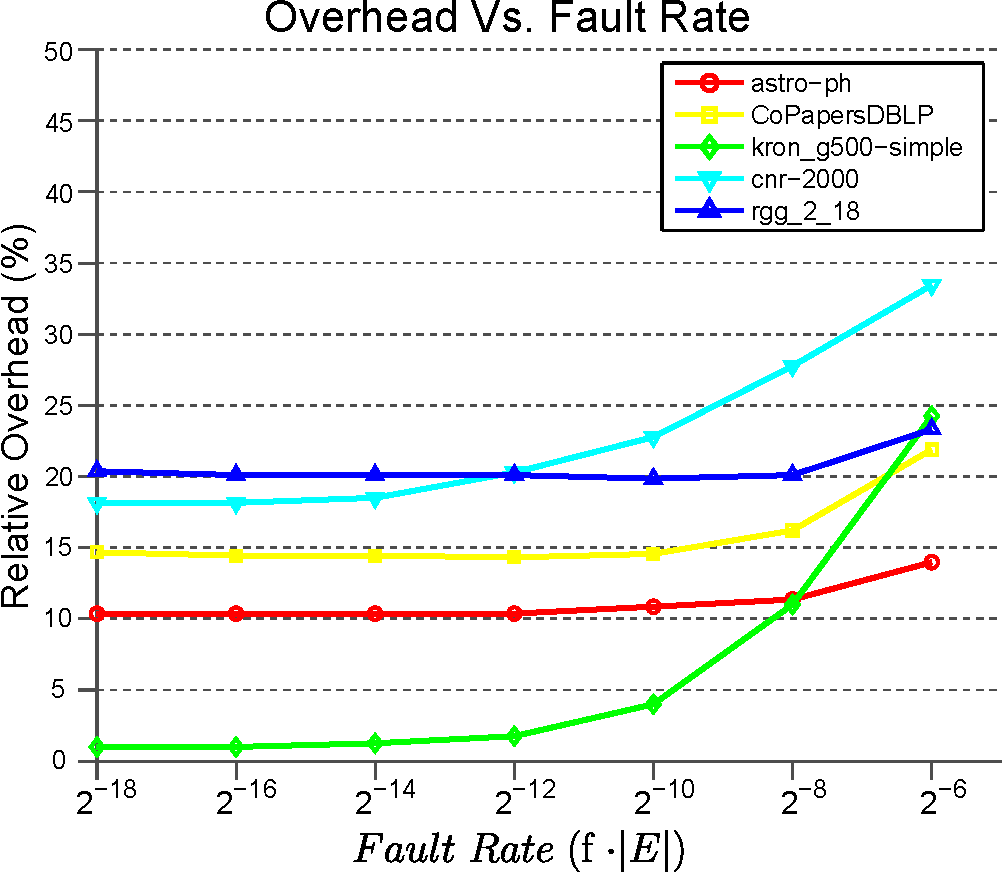
\includegraphics[height=.75\textheight]{plots/plot_overhead_fault-inked}

\lyxframeend{}
%%%%%%%%%%%%%%%%%%%%%%%%%%%%%%%%%%%%%%%%%%%%%%%%%%%%%%%%%


%%%%%%%%%%%%%%%%%%%%%%%%%%%%%%%%%%%%%%%%%%%%%%%%%%%%%%%%%
\lyxframe{Fault free overhead }
\centering
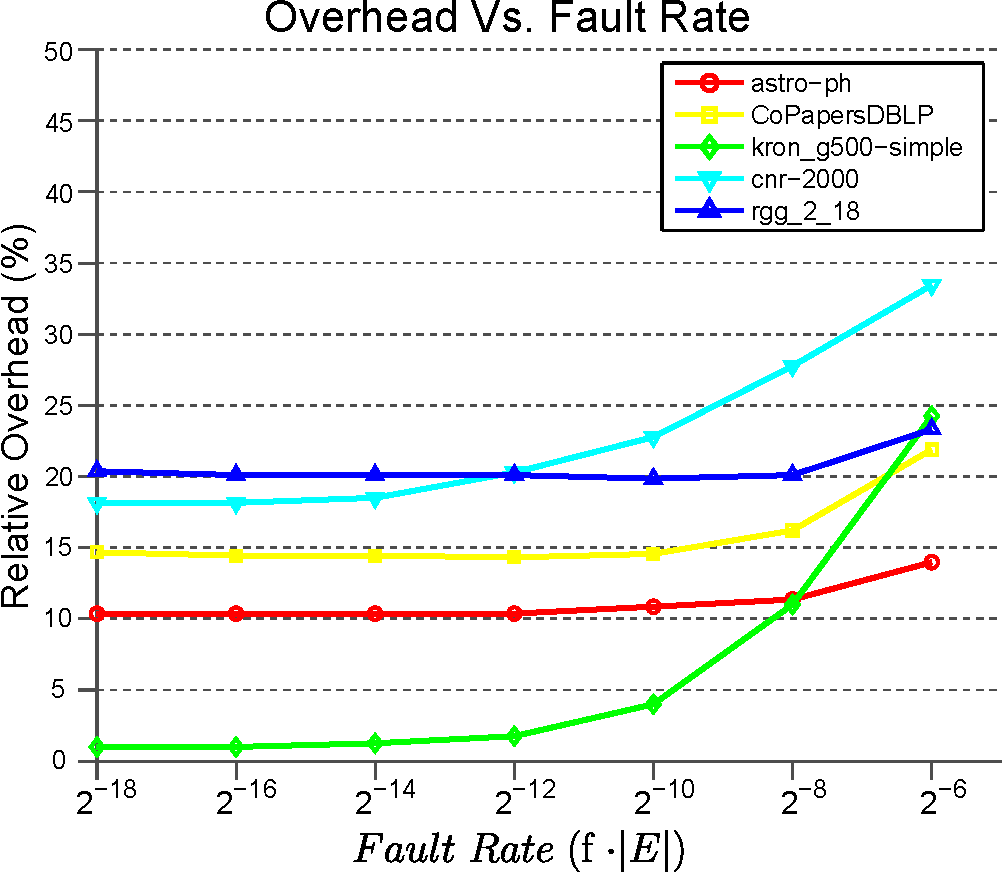
\includegraphics[height=.75\textheight]{plots/plot_overhead_fault-inked}

\lyxframeend{}
%%%%%%%%%%%%%%%%%%%%%%%%%%%%%%%%%%%%%%%%%%%%%%%%%%%%%%%%%

%%%%%%%%%%%%%%%%%%%%%%%%%%%%%%%%%%%%%%%%%%%%%%%%%%%%%%%%%
\lyxframe{Failure Rate for asynchronous case }
\centering
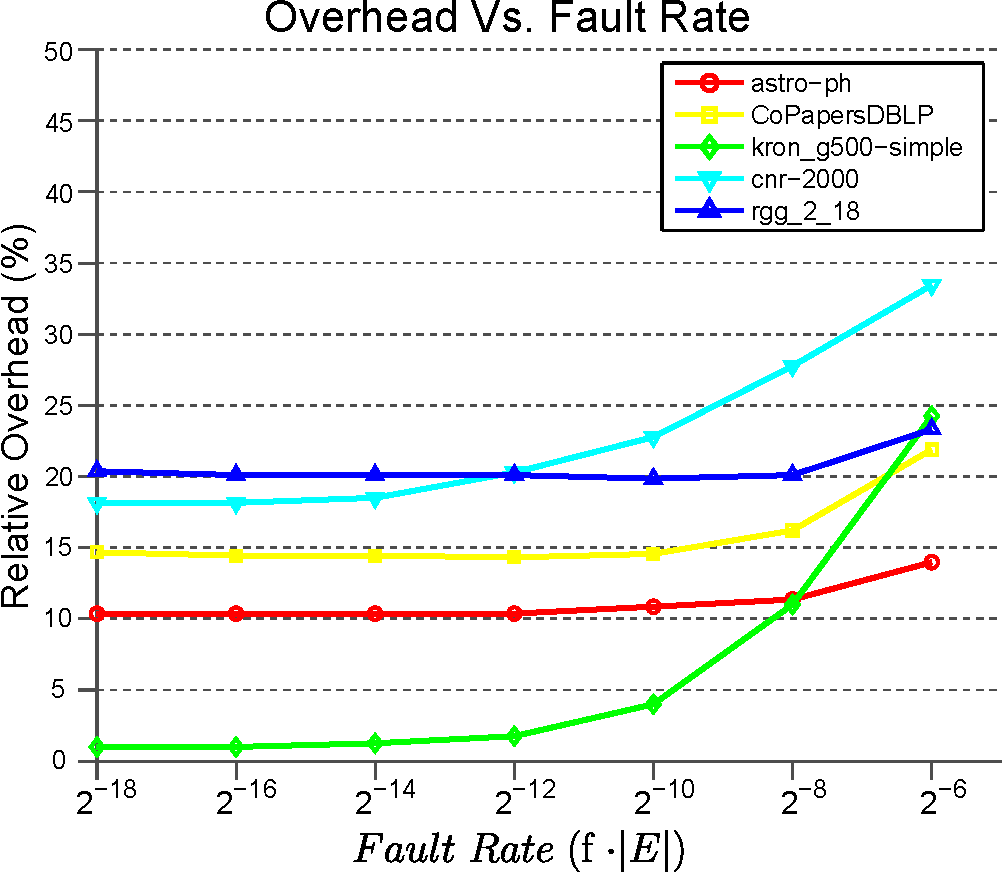
\includegraphics[height=.75\textheight]{plots/plot_overhead_fault-inked}

\lyxframeend{}
%%%%%%%%%%%%%%%%%%%%%%%%%%%%%%%%%%%%%%%%%%%%%%%%%%%%%%%%%


%%%%%%%%%%%%%%%%%%%%%%%%%%%%%%%%%%%%%%%%%%%%%%%%%%%%%%%%%
\lyxframe{Histogram for convergence}
\centering
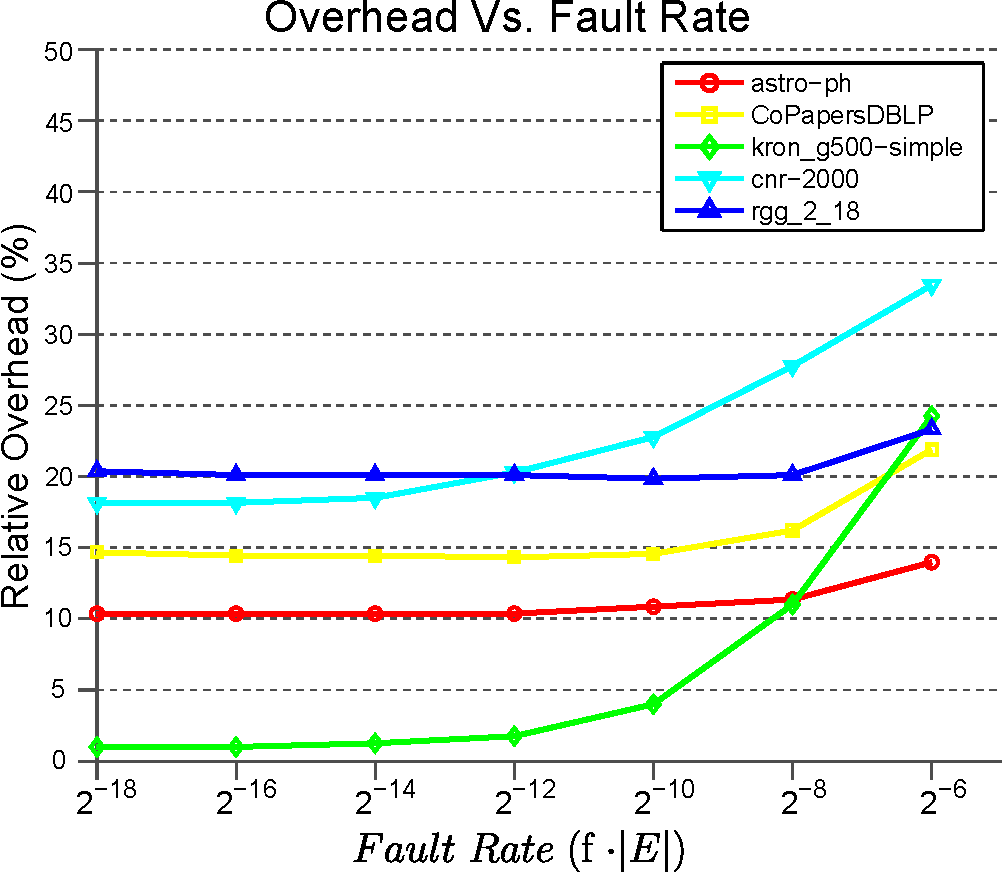
\includegraphics[height=.75\textheight]{plots/plot_overhead_fault-inked}
\lyxframeend{}
%%%%%%%%%%%%%%%%%%%%%%%%%%%%%%%%%%%%%%%%%%%%%%%%%%%%%%%%%



\label{sec:results}

\section{Related work}
Here goes the related work \cite{shantharam2012fault}.
\label{sec:related}

\section{Conclusion and future work}
\textbf{\emph{c}}\emph{onlusion} 
\begin{itemize}
\item what did we do 
\item what are implications 
\item where do we go from here 
\end{itemize}


\label{sec:conclusion}

\section{Acknowledgment}
\input{ack}

% \balance
\bibliographystyle{abbrv}
% \addbibresource{sao.bib}
\bibliography{sao}


\end{document}
